\documentclass[aspectratio=169,xcolor={dvipsnames}]{beamer}
\usepackage[utf8]{inputenc}
\usepackage[T1]{fontenc}
\usepackage[english]{babel}
\usepackage{textcomp}
\usepackage{upquote}
\usepackage{listings}
\usepackage{xcolor}
\usepackage{tikz}
\usepackage{graphicx}
\usepackage{amsmath}
\usepackage{hyperref}

% Definizione simboli personalizzati
\newcommand{\faCheckCircle}{$\checkmark$}
\newcommand{\faCode}{$\langle\rangle$}
\newcommand{\faLayerGroup}{[\,]}
\newcommand{\faSync}{$\circlearrowleft$}
\newcommand{\faTools}{$\star$}
\newcommand{\faExpand}{$\leftrightarrow$}
\newcommand{\faShieldAlt}{$\triangle$}
\newcommand{\faMobileAlt}{\texttt{M}}
\newcommand{\faLaptop}{\texttt{PC}}
\newcommand{\faMobile}{\texttt{M}}
\newcommand{\faDesktop}{\texttt{D}}
\newcommand{\faMicrochip}{$\mu$}
\newcommand{\faExclamationTriangle}{!}
\newcommand{\faPlug}{$\circ$}
\newcommand{\faDollarSign}{\$}
\newcommand{\faUsers}{\texttt{U}}
\newcommand{\faHeart}{$\heartsuit$}
\newcommand{\faEnvelope}{\texttt{@}}
\newcommand{\faGithub}{\texttt{Git}}
\newcommand{\faThumbsUp}{$\uparrow$}
\newcommand{\faTachometerAlt}{$\gg$}

\usetikzlibrary{shapes.geometric, arrows, positioning, shadows, calc}

% Beamer theme
\usetheme{Madrid}
\usecolortheme{default}
\setbeamercolor{structure}{fg=blue!70!black}
\setbeamercolor{title}{fg=white,bg=blue!70!black}
\setbeamercolor{frametitle}{fg=white,bg=blue!60!black}

% Listing settings for PHP
\lstdefinestyle{phpstyle}{
    language=PHP,
    basicstyle=\ttfamily\footnotesize,
    keywordstyle=\color{blue}\bfseries,
    commentstyle=\color{gray}\itshape,
    stringstyle=\color{red},
    numberstyle=\tiny\color{gray},
    numbers=left,
    stepnumber=1,
    numbersep=5pt,
    backgroundcolor=\color{gray!10},
    showspaces=false,
    showstringspaces=false,
    showtabs=false,
    frame=single,
    tabsize=2,
    captionpos=b,
    breaklines=true,
    breakatwhitespace=false,
    escapeinside={(*@}{@*)},
    morekeywords={class, function, public, private, protected, extends, require_once, define},
    upquote=true,
    literate=
        {'}{\textquotesingle}1
        {`}{\textasciigrave}1
        {"}{\textquotedbl}1
        {à}{{\`a}}1 {è}{{\`e}}1 {ì}{{\`{\i}}}1 {ò}{{\`o}}1 {ù}{{\`u}}1
        {À}{{\`A}}1 {È}{{\`E}}1 {Ì}{{\`I}}1 {Ò}{{\`O}}1 {Ù}{{\`U}}1
        {á}{{\'a}}1 {é}{{\'e}}1 {í}{{\'{\i}}}1 {ó}{{\'o}}1 {ú}{{\'u}}1
        {Á}{{\'A}}1 {É}{{\'E}}1 {Í}{{\'I}}1 {Ó}{{\'O}}1 {Ú}{{\'U}}1
        {€}{{\texteuro}}1 {£}{{\pounds}}1
        {->}{$\rightarrow$}2
        {=>}{$\Rightarrow$}2
}

\lstdefinestyle{sqlstyle}{
    language=SQL,
    basicstyle=\ttfamily\footnotesize,
    keywordstyle=\color{blue}\bfseries,
    commentstyle=\color{gray}\itshape,
    stringstyle=\color{orange},
    numbers=left,
    numberstyle=\tiny\color{gray},
    backgroundcolor=\color{gray!10},
    frame=single,
    breaklines=true,
    upquote=true,
    literate=
        {'}{\textquotesingle}1
        {`}{\textasciigrave}1
        {"}{\textquotedbl}1
}

\title{REST API in PHP 8}
\subtitle{Sviluppo di Servizi Web Moderni con MySQL}
\author{Prof. Fedeli Massimo Tutti i diritti riservati}
\institute{IIS Fermi Sacconi Ceci - Ascoli Piceno}
\date{\today}

\begin{document}

% ====================
% SLIDE 1: Title
% ====================
\begin{frame}
\titlepage
\end{frame}

% ====================
% SLIDE 2: Indice
% ====================
\begin{frame}{Indice}
\tableofcontents
\end{frame}

% ====================
% SECTION 1
% ====================
\section{Introduzione alle REST API}

% ====================
% SLIDE 3: Cosa sono le REST API
% ====================
\begin{frame}{Cosa sono le REST API?}
\begin{columns}[T]
\column{0.5\textwidth}
\textbf{REST} (Representational State Transfer) è uno stile architetturale per servizi web.

\vspace{0.5cm}

\textbf{Caratteristiche principali:}
\begin{itemize}
    \item \faCheckCircle\ Stateless (senza stato)
    \item \faCheckCircle\ Client-Server separation
    \item \faCheckCircle\ Cacheable
    \item \faCheckCircle\ Interfaccia uniforme
    \item \faCheckCircle\ Sistema a strati
\end{itemize}

\column{0.5\textwidth}
\begin{center}
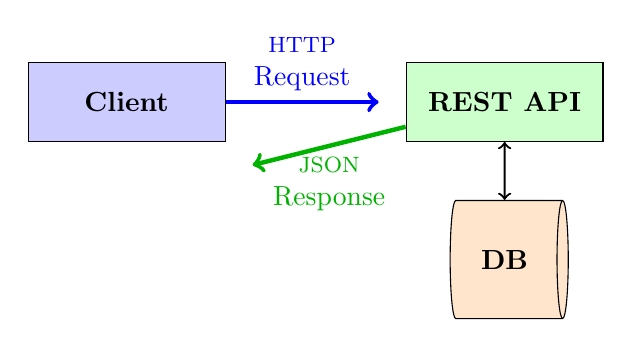
\begin{tikzpicture}[scale=0.8]
    % Client
    \node[draw, rectangle, fill=blue!20, minimum width=2.5cm, minimum height=1cm] (client) at (0,0) {\textbf{Client}};
    
    % Arrow
    \draw[->, ultra thick, blue] (client) -- node[above, align=center] {\footnotesize HTTP\\Request} (4,0);
    
    % Server
    \node[draw, rectangle, fill=green!20, minimum width=2.5cm, minimum height=1cm] (server) at (6,0) {\textbf{REST API}};
    
    % Arrow back
    \draw[->, ultra thick, green!70!black] (server) -- node[below, align=center] {\footnotesize JSON\\Response} (2,-1);
    
    % Database
    \node[draw, cylinder, fill=orange!20, minimum width=1.5cm, minimum height=1.5cm, shape aspect=0.3] (db) at (6,-2.5) {\textbf{DB}};
    
    \draw[<->, thick] (server) -- (db);
\end{tikzpicture}
\end{center}
\end{columns}
\end{frame}


\begin{frame}
	\begin{itemize}
\item REST è uno stile architetturale per la progettazione di sistemi distribuiti, in particolare servizi web. Non è una tecnologia in senso stretto né un protocollo, ma un insieme di principi che guidano la costruzione di API semplici, scalabili e manutenibili. 
\item REST non impone regole rigide, ma suggerisce buone pratiche.
\item Oggi REST è lo standard dominante per le API web, soprattutto in contesti microservizi, applicazioni web e mobile. Framework come Spring Boot, Django REST Framework, FastAPI o Express lo supportano nativamente.

	\end{itemize}
 \end{frame}



% ====================
% SLIDE 4: Vantaggi REST
% ====================
\begin{frame}{Vantaggi delle REST API}
\begin{columns}[T]
\column{0.5\textwidth}
\textbf{Per gli sviluppatori:}
\begin{itemize}
    \item \faCode\ Facilità di implementazione
    \item \faLayerGroup\ Separazione front-end/back-end
    \item \faSync\ Riutilizzabilità del codice
    \item \faTools\ Supporto di framework moderni
\end{itemize}

\vspace{0.5cm}
\textbf{Per le applicazioni:}
\begin{itemize}
    \item \faExpand\ Scalabilità
    \item \faShieldAlt\ Sicurezza migliorata
    \item \faMobileAlt\ Multi-piattaforma
\end{itemize}

\column{0.5\textwidth}
\begin{center}
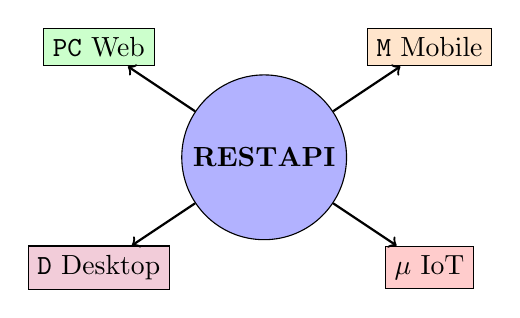
\begin{tikzpicture}[scale=0.7]
    % Central API
    \node[draw, circle, fill=blue!30, minimum size=2cm] (api) at (0,0) {\textbf{REST\\API}};
    
    % Web client
    \node[draw, rectangle, fill=green!20] (web) at (-3,2) {\faLaptop\ Web};
    \draw[->, thick] (api) -- (web);
    
    % Mobile client
    \node[draw, rectangle, fill=orange!20] (mobile) at (3,2) {\faMobile\ Mobile};
    \draw[->, thick] (api) -- (mobile);
    
    % Desktop
    \node[draw, rectangle, fill=purple!20] (desktop) at (-3,-2) {\faDesktop\ Desktop};
    \draw[->, thick] (api) -- (desktop);
    
    % IoT
    \node[draw, rectangle, fill=red!20] (iot) at (3,-2) {\faMicrochip\ IoT};
    \draw[->, thick] (api) -- (iot);
\end{tikzpicture}
\end{center}

\vspace{0.3cm}
\small\textit{Un unica API per tutti i client}
\end{columns}
\end{frame}

% ====================
% SLIDE 5: Metodi HTTP
% ====================
\begin{frame}{Metodi HTTP nelle REST API}
\begin{center}
\begin{tabular}{|c|l|l|}
\hline
\textbf{Metodo} & \textbf{Operazione} & \textbf{Esempio} \\
\hline
\textcolor{blue}{\textbf{GET}} & Recupera risorse & \texttt{GET /users} \\
& & \texttt{GET /users/5} \\
\hline
\textcolor{green!70!black}{\textbf{POST}} & Crea nuove risorse & \texttt{POST /users} \\
\hline
\textcolor{orange}{\textbf{PUT}} & Aggiorna risorse (completo) & \texttt{PUT /users/5} \\
\hline
\textcolor{purple}{\textbf{PATCH}} & Aggiorna risorse (parziale) & \texttt{PATCH /users/5} \\
\hline
\textcolor{red}{\textbf{DELETE}} & Elimina risorse & \texttt{DELETE /users/5} \\
\hline
\end{tabular}
\end{center}

REST impone una semantica precisa ai metodi HTTP.

\begin{block}{CRUD Operations}
\begin{itemize}
    \item \textbf{C}reate $\rightarrow$ POST
    \item \textbf{R}ead $\rightarrow$ GET
    \item \textbf{U}pdate $\rightarrow$ PUT/PATCH
    \item \textbf{D}elete $\rightarrow$ DELETE
\end{itemize}
\end{block}
\end{frame}

% ====================
% SLIDE 6: Codici di stato HTTP
% ====================
\begin{frame}{Codici di Stato HTTP}
\begin{columns}[T]
\column{0.5\textwidth}
\textbf{2xx - Successo}
\begin{itemize}
    \item \textcolor{green!70!black}{200 OK} - Richiesta riuscita
    \item \textcolor{green!70!black}{201 Created} - Risorsa creata
    \item \textcolor{green!70!black}{204 No Content} - Successo senza contenuto
\end{itemize}

\vspace{0.3cm}
\textbf{4xx - Errori Client}
\begin{itemize}
    \item \textcolor{orange}{400 Bad Request} - Richiesta malformata
    \item \textcolor{orange}{401 Unauthorized} - Non autenticato
    \item \textcolor{orange}{404 Not Found} - Risorsa non trovata
    \item \textcolor{orange}{422 Unprocessable} - Dati non validi
\end{itemize}

\column{0.5\textwidth}
\textbf{5xx - Errori Server}
\begin{itemize}
    \item \textcolor{red}{500 Internal Error} - Errore del server
    \item \textcolor{red}{503 Unavailable} - Servizio non disponibile
\end{itemize}

\vspace{0.5cm}
\begin{alertblock}{Best Practice}
Utilizzare sempre i codici di stato appropriati per comunicare chiaramente il risultato dell'operazione.
\end{alertblock}
\end{columns}
\end{frame}

% ====================
% SECTION 2	<?php
// Controller/Api/BaseController.php

class BaseController
{
	/**
	* Magic method per gestire chiamate a metodi inesistenti
	*/
	public function __call($name, $arguments)
	{
		$this->sendOutput('', 
		array('HTTP/1.1 404 Not Found'));
	}
	
% ====================
\section{Architettura del Progetto}

% ====================
% SLIDE 7: Struttura del progetto
% ====================
\begin{frame}[fragile]{Struttura del Progetto}
\begin{columns}[T]
\column{0.45\textwidth}
\begin{lstlisting}[style=phpstyle, basicstyle=\ttfamily\tiny]
rest-api-php/
|-- index.php
|-- inc/
|   |-- config.php
|   |-- bootstrap.php
|-- Model/
|   |-- Database.php
|   |-- UserModel.php
|-- Controller/
    |-- Api/
        |-- BaseController.php
        |-- UserController.php
\end{lstlisting}

\column{0.55\textwidth}
\textbf{Componenti principali:}
\begin{itemize}
    \item \textbf{index.php}: Entry point dell'applicazione
    \item \textbf{inc/}: File di configurazione e bootstrap
    \item \textbf{Model/}: Data Access Layer
    \item \textbf{Controller/}: Logica di business
\end{itemize}

\vspace{0.3cm}
\begin{block}{Pattern MVC}
Adottiamo il pattern Model-View-Controller per separare le responsabilità e migliorare la manutenibilità del codice.
\end{block}
\end{columns}
\end{frame}

% ====================
% SLIDE 8: Pattern MVC
% ====================
\begin{frame}{Pattern MVC nell'API REST}
\begin{center}
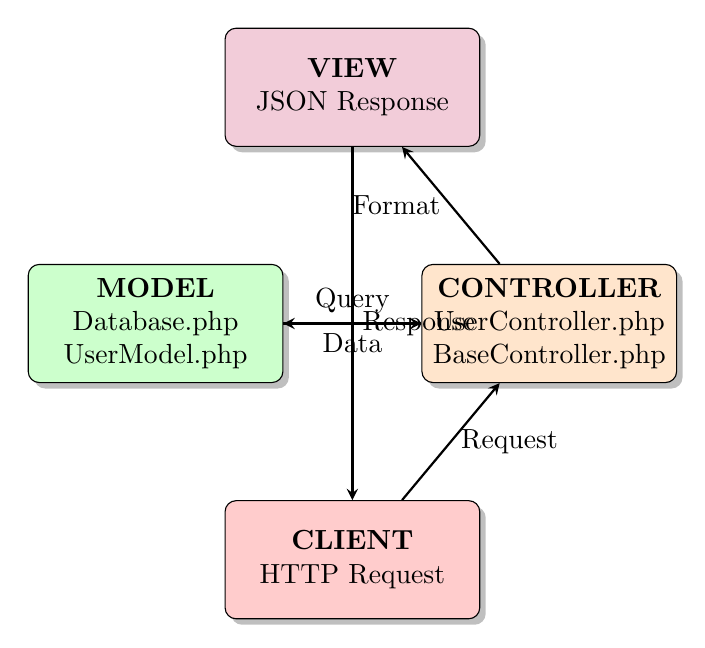
\begin{tikzpicture}[node distance=2cm, auto]
    % Styles
    \tikzstyle{block} = [rectangle, draw, fill=blue!20, text width=3cm, text centered, rounded corners, minimum height=1.5cm, drop shadow]
    \tikzstyle{arrow} = [thick,->,>=stealth]
    
    % Model
    \node[block, fill=green!20] (model) at (0,0) {\textbf{MODEL}\\Database.php\\UserModel.php};
    
    % Controller
    \node[block, fill=orange!20] (controller) at (5,0) {\textbf{CONTROLLER}\\UserController.php\\BaseController.php};
    
    % View (JSON)
    \node[block, fill=purple!20] (view) at (2.5,3) {\textbf{VIEW}\\JSON Response};
    
    % Client
    \node[block, fill=red!20] (client) at (2.5,-3) {\textbf{CLIENT}\\HTTP Request};
    
    % Arrows
    \draw[arrow] (client) -- node[right] {Request} (controller);
    \draw[arrow] (controller) -- node[above] {Query} (model);
    \draw[arrow] (model) -- node[below] {Data} (controller);
    \draw[arrow] (controller) -- node[left] {Format} (view);
    \draw[arrow] (view) -- node[right] {Response} (client);
\end{tikzpicture}
\end{center}
\end{frame}

% ====================
% SECTION 3
% ====================
\section{Configurazione Database}

% ====================
% SLIDE 9: Creazione Database
% ====================
\begin{frame}[fragile]{Creazione del Database MySQL}
\textbf{Step 1: Creare il database}
\begin{lstlisting}[style=sqlstyle]
CREATE DATABASE rest_api_php;
\end{lstlisting}

\vspace{0.3cm}
\textbf{Step 2: Creare la tabella users}
\begin{lstlisting}[style=sqlstyle, basicstyle=\ttfamily\scriptsize]
USE rest_api_php;

CREATE TABLE `users` (
  `user_id` bigint(20) unsigned NOT NULL AUTO_INCREMENT,
  `username` varchar(60) COLLATE utf8mb4_unicode_ci 
              NOT NULL DEFAULT '',
  `user_email` varchar(100) COLLATE utf8mb4_unicode_ci 
                NOT NULL DEFAULT '',
  `user_status` int(11) NOT NULL DEFAULT '0',
  PRIMARY KEY (`user_id`)
) ENGINE=InnoDB DEFAULT CHARSET=utf8mb4 
  COLLATE=utf8mb4_unicode_ci;
\end{lstlisting}
\end{frame}

% ====================
% SLIDE 10: Popolamento Database
% ====================
\begin{frame}[fragile]{Popolamento del Database}
\textbf{Inserimento dati di esempio:}
\begin{lstlisting}[style=sqlstyle]
INSERT INTO `users`
  (`user_id`, `username`, `user_email`, `user_status`) 
VALUES 
  (1, 'Gina', 'ginaverdi@gmail.com', 0),
  (2, 'Mario', 'mario.rossi@email.com', 1),
  (3, 'Laura', 'laura.bianchi@email.com', 1),
  (4, 'Paolo', 'paolo.verdi@email.com', 0),
  (5, 'Sara', 'sara.neri@email.com', 1);
\end{lstlisting}

\vspace{0.3cm}
\begin{alertblock}{Nota}
Il campo \texttt{user\_status} può indicare se l'utente è attivo (1) o inattivo (0).
\end{alertblock}
\end{frame}

% ====================
% SLIDE 11: Schema ER
% ====================
\begin{frame}{Schema Entity-Relationship}
\begin{center}
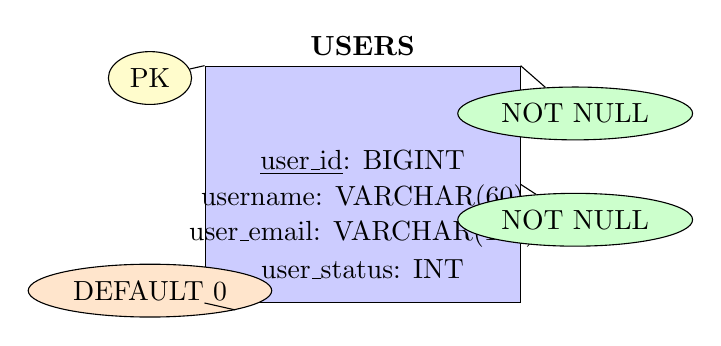
\begin{tikzpicture}[scale=0.9]
    % Entity Users
    \node[draw, rectangle, fill=blue!20, minimum width=4cm, minimum height=3cm] (users) at (0,0) {};
    \node[above] at (users.north) {\textbf{USERS}};
    
    \node[align=left] at (0,0.3) {\underline{user\_id}: BIGINT};
    \node[align=left] at (0,-0.2) {username: VARCHAR(60)};
    \node[align=left] at (0,-0.7) {user\_email: VARCHAR(100)};
    \node[align=left] at (0,-1.2) {user\_status: INT};
    
    % Properties
    \node[draw, ellipse, fill=yellow!20] (pk) at (-3,1.5) {PK};
    \draw[-] (pk) -- (users.north west);
    
    \node[draw, ellipse, fill=green!20] (nn1) at (3,1) {NOT NULL};
    \draw[-] (nn1) -- (users.north east);
    
    \node[draw, ellipse, fill=green!20] (nn2) at (3,-0.5) {NOT NULL};
    \draw[-] (nn2) -- (users.east);
    
    \node[draw, ellipse, fill=orange!20] (def) at (-3,-1.5) {DEFAULT 0};
    \draw[-] (def) -- (users.south west);
\end{tikzpicture}
\end{center}

\vspace{0.3cm}
\small\textbf{Vincoli:}
\begin{itemize}
    \item user\_id è la chiave primaria (AUTO\_INCREMENT)
    \item username e user\_email sono obbligatori
    \item user\_status ha valore predefinito 0
\end{itemize}
\end{frame}

% ====================
% SECTION 4
% ====================
\section{Implementazione Models}

% ====================
% SLIDE 12: File config.php
% ====================
\begin{frame}[fragile]{File di Configurazione - config.php}
\begin{lstlisting}[style=phpstyle]
<?php
// inc/config.php

define("DB_HOST", "localhost");
define("DB_USERNAME", "root");
define("DB_PASSWORD", "");
define("DB_DATABASE_NAME", "rest_api_php");
?>
\end{lstlisting}

\vspace{0.5cm}
\begin{block}{Best Practice}
\begin{itemize}
    \item Separare sempre la configurazione dal codice
    \item Utilizzare variabili d'ambiente in produzione
    \item Non versionare mai le credenziali su Git
    \item Considerare l'uso di file .env
\end{itemize}
\end{block}
\end{frame}

% ====================
% SLIDE 13: File bootstrap.php
% ====================
\begin{frame}[fragile]{File Bootstrap}
\begin{lstlisting}[style=phpstyle]
<?php
// inc/bootstrap.php

define("PROJECT_ROOT_PATH", __DIR__ . "/../");

// Include main configuration file
require_once PROJECT_ROOT_PATH . "/inc/config.php";

// Include the base controller file
require_once PROJECT_ROOT_PATH . 
    "/Controller/Api/BaseController.php";

// Include the user model file
require_once PROJECT_ROOT_PATH . 
    "/Model/UserModel.php";
?>
\end{lstlisting}

\vspace{0.3cm}
\small\textbf{Il file bootstrap} carica tutti i componenti necessari all'avvio dell'applicazione, definisce il path root e include i file fondamentali.
\end{frame}

% ====================
% SLIDE 14: Classe Database
% ====================
\begin{frame}[fragile]{Classe Database - Parte 1}
\begin{lstlisting}[style=phpstyle, basicstyle=\ttfamily\scriptsize]
<?php
// Model/Database.php

class Database
{
    protected $connection = null;

    public function __construct()
    {
        try {
            $this->connection = new mysqli(
                DB_HOST, 
                DB_USERNAME, 
                DB_PASSWORD, 
                DB_DATABASE_NAME
            );
            
            if (mysqli_connect_errno()) {
                throw new Exception(
                    "Could not connect to database."
                );
            }
        } catch (Exception $e) {
            throw new Exception($e->getMessage());
        }
    }
\end{lstlisting}
\end{frame}

% ====================
% SLIDE 15: Classe Database - Metodi
% ====================

\begin{frame}[fragile]{Classe Database - Parte 2}
	\begin{lstlisting}[style=phpstyle, basicstyle=\ttfamily\scriptsize]
		public function select($query = "", $params = [])
		{
			try {
				$stmt = $this->executeStatement($query, $params);
				$result = $stmt->get_result()
				->fetch_all(MYSQLI_ASSOC);
				$stmt->close();
				return $result;
			} catch (Exception $e) {
				throw new Exception($e->getMessage());
			}
		}
		
\end{lstlisting}
\end{frame}


\begin{frame}[fragile]{Classe Database - Parte 2}
	\begin{lstlisting}[style=phpstyle, basicstyle=\ttfamily\scriptsize]
			
		private function executeStatement($query = "", $params = [])
		{
			try {
				$stmt = $this->connection->prepare($query);
				if ($stmt === false) {
					throw new Exception(
					"Unable to prepare statement: " . $query
					);
				}
				if ($params) {
					$stmt->bind_param($params[0], $params[1]);
				}
				$stmt->execute();
				return $stmt;
			} catch (Exception $e) {
				throw new Exception($e->getMessage());
			}
		}
	}
\end{lstlisting}
\end{frame}


% ====================
% SLIDE 16: Caratteristiche Database Class
% ====================
\begin{frame}{Caratteristiche della Classe Database}
\begin{columns}[T]
\column{0.5\textwidth}
\textbf{Funzionalità:}
\begin{itemize}
    \item \faPlug\ Gestione connessione MySQL
    \item \faShieldAlt\ Prepared Statements (SQL Injection)
    \item \faExclamationTriangle\ Gestione eccezioni
    \item \faLayerGroup\ Pattern Template per estensione
\end{itemize}

\vspace{0.3cm}
\textbf{Metodi principali:}
\begin{itemize}
    \item \texttt{\_\_construct()}: Stabilisce connessione
    \item \texttt{select()}: Esegue query SELECT
    \item \texttt{executeStatement()}: Prepara ed esegue statement
\end{itemize}

\column{0.5\textwidth}
\begin{alertblock}{Sicurezza}
L'uso di \textbf{Prepared Statements} con \texttt{bind\_param()} protegge da attacchi SQL Injection parametrizzando le query.
\end{alertblock}

\vspace{0.3cm}
\begin{exampleblock}{Estensibilità}
La classe è progettata per essere estesa da Model specifici (UserModel, ProductModel, ecc.) che implementano la logica di business.
\end{exampleblock}
\end{columns}
\end{frame}

% ====================
% SLIDE 17: UserModel
% ====================
\begin{frame}[fragile]{Classe UserModel}
\begin{lstlisting}[style=phpstyle]
<?php
// Model/UserModel.php

require_once PROJECT_ROOT_PATH . "/Model/Database.php";

class UserModel extends Database
{
    public function getUsers($limit)
    {
        return $this->select(
            "SELECT * FROM users 
             ORDER BY user_id ASC 
             LIMIT ?",
            ["i", $limit]
        );
    }
}
?>
\end{lstlisting}

\vspace{0.3cm}
\begin{itemize}
    \item \textbf{Estende Database}: Eredita metodi di connessione e query
    \item \textbf{getUsers(\$limit)}: Recupera utenti con limite parametrizzato
    \item \textbf{"i"}: Indica che \$limit è di tipo integer nel binding
\end{itemize}
\end{frame}

% ====================
% SECTION 5
% ====================
\section{Implementazione Controllers}

% ====================
% SLIDE 18: BaseController
% ====================
\begin{frame}[fragile]{Classe BaseController - Parte 1}
\begin{lstlisting}[style=phpstyle, basicstyle=\ttfamily\scriptsize]
<?php
// Controller/Api/BaseController.php

class BaseController
{
    /**
     * Magic method per gestire chiamate a metodi inesistenti
     */
    public function __call($name, $arguments)
    {
        $this->sendOutput('', 
            array('HTTP/1.1 404 Not Found'));
    }

\end{lstlisting}
\end{frame}


\begin{frame}[fragile]{Classe BaseController - Parte 1}
	\begin{lstlisting}[style=phpstyle, basicstyle=\ttfamily\scriptsize]
	
			/**
			* Estrae i segmenti dall'URI
			*/
			protected function getUriSegments()
			{
				$uri = parse_url($_SERVER['REQUEST_URI'], 
				PHP_URL_PATH);
				$uri = explode('/', $uri);
				return $uri;
			}
		\end{lstlisting}
	\end{frame}


% ====================
% SLIDE 19: BaseController - Parte 2
% ====================
\begin{frame}[fragile]{Classe BaseController - Parte 2}
\begin{lstlisting}[style=phpstyle, basicstyle=\ttfamily\scriptsize]
    /**
     * Recupera parametri della query string
     */
    protected function getQueryStringParams()
    {
        parse_str($_SERVER['QUERY_STRING'], $query);
        return $query;
    }

    /**
     * Invia l'output JSON al client
     */
    protected function sendOutput($data, 
                                   $httpHeaders = array())
    {
        header_remove('Set-Cookie');
        
        if (is_array($httpHeaders) && count($httpHeaders)) {
            foreach ($httpHeaders as $httpHeader) {
                header($httpHeader);
            }
        }
        
        echo $data;
        exit;
    }
}
\end{lstlisting}
\end{frame}

% ====================
% SLIDE 20: Metodi BaseController
% ====================
\begin{frame}{Metodi della Classe BaseController}
%\begin{center}
%\begin{tikzpicture}[node distance=1.5cm]
%    \tikzstyle{method} = [rectangle, draw, fill=blue!20, text width=4cm, text centered, rounded corners, minimum height=1cm]
%    
%    \node[method] (call) at (0,3) {\textbf{\_\_call()}\\Gestisce metodi non esistenti};
%    
%    \node[method] (uri) at (0,1.5) {\textbf{getUriSegments()}\\Estrae segmenti URI};
%    
%    \node[method] (query) at (0,0) {\textbf{getQueryStringParams()}\\Recupera parametri query};
%    
%    \node[method] (output) at (0,-1.5) {\textbf{sendOutput()}\\Invia risposta HTTP};
%    
%    % Central controller
%    \node[draw, ellipse, fill=orange!30, minimum width=3cm, minimum height=2cm] (base) at (6,0.75) {\Large\textbf{Base\\Controller}};
%    
%    \draw[->, thick] (uri) -- (base);
%    \draw[->, thick] (query) -- (base);
%    \draw[->, thick] (output) -- (base);
%    \draw[->, thick] (call) -- (base);
%\end{tikzpicture}
%\end{center}

\vspace{0.2cm}
\small Questi metodi forniscono funzionalità comuni a tutti i controller dell API.
\end{frame}

% ====================
% SLIDE 21: UserController - Parte 1
% ====================
\begin{frame}[fragile]{Classe UserController - Parte 1}
\begin{lstlisting}[style=phpstyle, basicstyle=\ttfamily\tiny]
<?php
// Controller/Api/UserController.php

class UserController extends BaseController
{
    /**
     * Endpoint: /user/list
     * Restituisce l'elenco degli utenti
     */
    public function listAction()
    {
        $strErrorDesc = '';
        $requestMethod = $_SERVER["REQUEST_METHOD"];
        $arrQueryStringParams = $this->getQueryStringParams();

        if (strtoupper($requestMethod) == 'GET') {
            try {
                $userModel = new UserModel();
                $intLimit = 10;
                
                if (isset($arrQueryStringParams['limit']) && 
                    $arrQueryStringParams['limit']) {
                    $intLimit = $arrQueryStringParams['limit'];
                }

                $arrUsers = $userModel->getUsers($intLimit);
                $responseData = json_encode($arrUsers);
\end{lstlisting}
\end{frame}

% ====================
% SLIDE 22: UserController - Parte 2
% ====================
\begin{frame}[fragile]{Classe UserController - Parte 2}
\begin{lstlisting}[style=phpstyle, basicstyle=\ttfamily\tiny]
            } catch (Error $e) {
                $strErrorDesc = $e->getMessage() . 
                    'Something went wrong! Please contact support.';
                $strErrorHeader = 'HTTP/1.1 500 Internal Server Error';
            }
        } else {
            $strErrorDesc = 'Method not supported';
            $strErrorHeader = 'HTTP/1.1 422 Unprocessable Entity';
        }
        
        // Invia output
        if (!$strErrorDesc) {
            $this->sendOutput(
                $responseData,
                array('Content-Type: application/json', 
                      'HTTP/1.1 200 OK')
            );
        } else {
            $this->sendOutput(
                json_encode(array('error' => $strErrorDesc)),
                array('Content-Type: application/json', 
                      $strErrorHeader)
            );
        }
    }
}
\end{lstlisting}
\end{frame}

% ====================
% SLIDE 23: Flusso UserController
% ====================
\begin{frame}{Flusso di Esecuzione in UserController}
\begin{center}
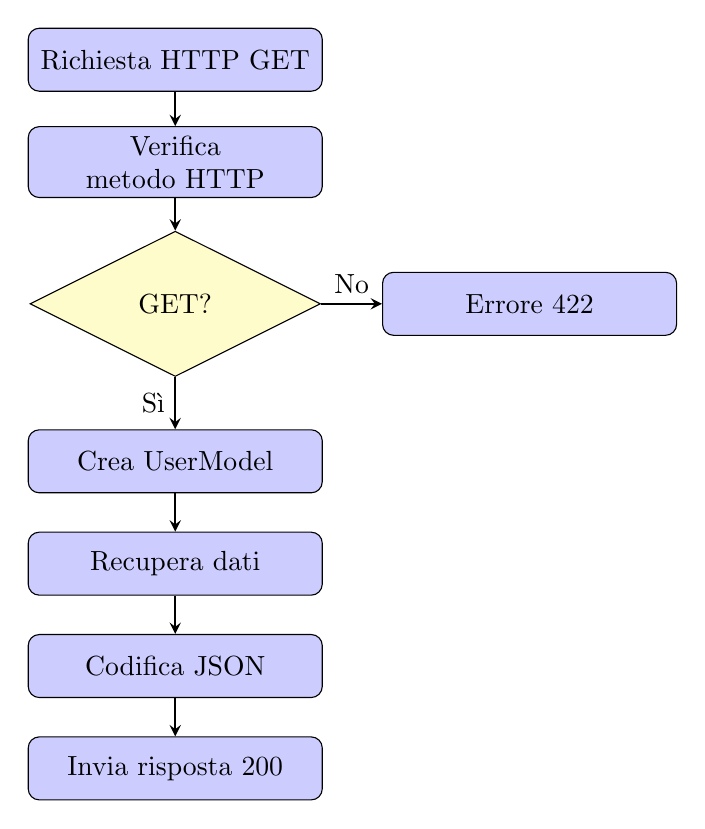
\begin{tikzpicture}[node distance=1.3cm, auto]
    \tikzstyle{block} = [rectangle, draw, fill=blue!20, text width=3.5cm, text centered, rounded corners, minimum height=0.8cm]
    \tikzstyle{decision} = [diamond, draw, fill=yellow!20, text width=2.5cm, text centered, aspect=2]
    \tikzstyle{arrow} = [thick,->,>=stealth]
    
    \node[block] (start) at (0,0) {Richiesta HTTP GET};
    \node[block, below of=start] (check) {Verifica metodo HTTP};
    \node[decision, below of=check, node distance=1.8cm] (isget) {GET?};
    \node[block, below of=isget, node distance=2cm] (model) {Crea UserModel};
    \node[block, below of=model] (get) {Recupera dati};
    \node[block, below of=get] (encode) {Codifica JSON};
    \node[block, below of=encode] (send) {Invia risposta 200};
    \node[block, right of=isget, node distance=4.5cm] (error) {Errore 422};
    
    \draw[arrow] (start) -- (check);
    \draw[arrow] (check) -- (isget);
    \draw[arrow] (isget) -- node[left] {Sì} (model);
    \draw[arrow] (isget) -- node[above] {No} (error);
    \draw[arrow] (model) -- (get);
    \draw[arrow] (get) -- (encode);
    \draw[arrow] (encode) -- (send);
\end{tikzpicture}
\end{center}
\end{frame}

% ====================
% SECTION 6
% ====================
\section{Entry Point e Routing}

% ====================
% SLIDE 24: File index.php
% ====================
\begin{frame}[fragile]{Entry Point - index.php}
\begin{lstlisting}[style=phpstyle, basicstyle=\ttfamily\scriptsize]
<?php
// index.php

require __DIR__ . "/inc/bootstrap.php";

$uri = parse_url($_SERVER['REQUEST_URI'], PHP_URL_PATH);
$uri = explode('/', $uri);

// Validazione URI
if ((isset($uri[2]) && $uri[2] != 'user') || 
    !isset($uri[3])) {
    header("HTTP/1.1 404 Not Found");
    exit();
}

// Carica il controller appropriato
require PROJECT_ROOT_PATH . 
    "/Controller/Api/UserController.php";

$objFeedController = new UserController();
$strMethodName = $uri[3] . 'Action';
$objFeedController->{$strMethodName}();
?>
\end{lstlisting}
\end{frame}

% ====================
% SLIDE 25: Analisi URI Routing
% ====================
\begin{frame}{Analisi del Routing URI}
\textbf{Struttura URI:}
\begin{center}
\Large
\texttt{http://localhost/index.php/\textcolor{blue}{user}/\textcolor{red}{list}?limit=20}
\end{center}

\vspace{0.5cm}

\begin{columns}[T]
\column{0.5\textwidth}
\textbf{Componenti URI:}
\begin{itemize}
    \item \texttt{\$uri[0]} $\rightarrow$ '' (vuoto)
    \item \texttt{\$uri[1]} $\rightarrow$ 'index.php'
    \item \texttt{\$uri[2]} $\rightarrow$ \textcolor{blue}{'user'} (modulo)
    \item \texttt{\$uri[3]} $\rightarrow$ \textcolor{red}{'list'} (metodo)
\end{itemize}

\column{0.5\textwidth}
\textbf{Processo:}
\begin{enumerate}
    \item Parse dell'URI
    \item Validazione modulo
    \item Caricamento controller
    \item Invocazione metodo dinamico
\end{enumerate}

\vspace{0.3cm}
\small\texttt{\$uri[3] . 'Action'} $\rightarrow$ \texttt{listAction()}
\end{columns}
\end{frame}

% ====================
% SLIDE 26: Routing Diagram
% ====================
\begin{frame}{Diagramma del Sistema di Routing}
\begin{center}
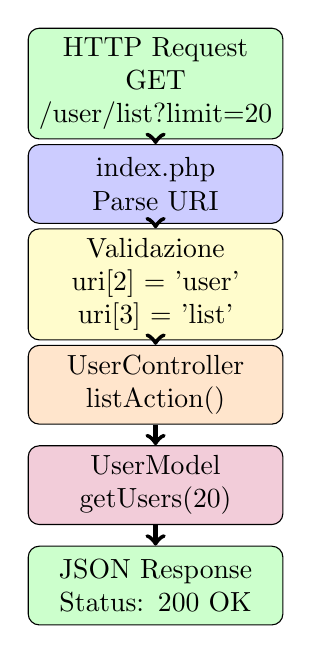
\begin{tikzpicture}[scale=0.85]
    \tikzstyle{block} = [rectangle, draw, fill=blue!20, text width=3cm, text centered, rounded corners, minimum height=1cm]
    
    % Request
    \node[block, fill=green!20] (req) at (0,4) {HTTP Request\\GET /user/list?limit=20};
    
    % index.php
    \node[block] (index) at (0,2.5) {index.php\\Parse URI};
    
    % Validation
    \node[block, fill=yellow!20] (valid) at (0,1) {Validazione\\uri[2] = 'user'\\uri[3] = 'list'};
    
    % Controller
    \node[block, fill=orange!20] (ctrl) at (0,-0.5) {UserController\\listAction()};
    
    % Model
    \node[block, fill=purple!20] (model) at (0,-2) {UserModel\\getUsers(20)};
    
    % Response
    \node[block, fill=green!20] (resp) at (0,-3.5) {JSON Response\\Status: 200 OK};
    
    % Arrows
    \draw[->, ultra thick] (req) -- (index);
    \draw[->, ultra thick] (index) -- (valid);
    \draw[->, ultra thick] (valid) -- (ctrl);
    \draw[->, ultra thick] (ctrl) -- (model);
    \draw[->, ultra thick] (model) -- (resp);
\end{tikzpicture}
\end{center}
\end{frame}

% ====================
% SECTION 7
% ====================
\section{Testing e Utilizzo}

% ====================
% SLIDE 27: Chiamata API
% ====================
\begin{frame}[fragile]{Chiamare l'API REST}
\textbf{Sintassi generale:}
\begin{center}
\Large
\texttt{http://localhost/index.php/\{MODULE\}/\{METHOD\}?\{PARAMS\}}
\end{center}

\vspace{0.5cm}

\textbf{Esempio pratico:}
\begin{lstlisting}[style=phpstyle, basicstyle=\ttfamily\small]
http://localhost/index.php/user/list?limit=20
\end{lstlisting}

\vspace{0.5cm}

\textbf{Parametri disponibili:}
\begin{itemize}
    \item \texttt{limit}: Numero massimo di utenti da recuperare
    \item Default: 10 utenti se non specificato
\end{itemize}

\vspace{0.3cm}
\begin{exampleblock}{Testing Tools}
Utilizzare strumenti come:
\begin{itemize}
    \item Browser web (per GET)
    \item Postman
    \item cURL
    \item Insomnia
\end{itemize}
\end{exampleblock}
\end{frame}

% ====================
% SLIDE 28: Risposta JSON
% ====================
\begin{frame}[fragile]{Formato della Risposta JSON}
\textbf{Risposta di successo:}
\begin{lstlisting}[style=phpstyle, basicstyle=\ttfamily\tiny]
[
    {
        "user_id": "1",
        "username": "Gina",
        "user_email": "ginaverdi@gmail.com",
        "user_status": "0"
    },
    {
        "user_id": "2",
        "username": "Mario",
        "user_email": "mario.rossi@email.com",
        "user_status": "1"
    },
    {
        "user_id": "3",
        "username": "Laura",
        "user_email": "laura.bianchi@email.com",
        "user_status": "1"
    }
]
\end{lstlisting}

\vspace{0.3cm}
\small\textbf{Headers della risposta:}
\begin{itemize}
    \item \texttt{Content-Type: application/json}
    \item \texttt{HTTP/1.1 200 OK}
\end{itemize}
\end{frame}

% ====================
% SLIDE 29: Gestione Errori
% ====================
\begin{frame}[fragile]{Gestione degli Errori}
\textbf{Errore metodo non supportato (422):}
\begin{lstlisting}[style=phpstyle, basicstyle=\ttfamily\small]
{
    "error": "Method not supported"
}
\end{lstlisting}

\vspace{0.3cm}
\textbf{Errore interno del server (500):}
\begin{lstlisting}[style=phpstyle, basicstyle=\ttfamily\small]
{
    "error": "Something went wrong! 
              Please contact support."
}
\end{lstlisting}

\vspace{0.3cm}
\textbf{Risorsa non trovata (404):}
\begin{lstlisting}[style=phpstyle, basicstyle=\ttfamily\small]
HTTP/1.1 404 Not Found
\end{lstlisting}

\vspace{0.3cm}
\small Ogni tipo di errore restituisce il codice HTTP appropriato e un messaggio descrittivo in formato JSON.
\end{frame}

% ====================
% SLIDE 30: Testing con cURL
% ====================
\begin{frame}[fragile]{Testing con cURL}
\textbf{GET Request - Recupera 5 utenti:}
\begin{lstlisting}[language=bash, basicstyle=\ttfamily\small]
curl -X GET "http://localhost/index.php/user/list?limit=5"
\end{lstlisting}

\vspace{0.3cm}
\textbf{GET Request con headers visibili:}
\begin{lstlisting}[language=bash, basicstyle=\ttfamily\tiny]
curl -i -X GET "http://localhost/index.php/user/list?limit=10"
\end{lstlisting}

\vspace{0.3cm}
\textbf{Test metodo non supportato:}
\begin{lstlisting}[language=bash, basicstyle=\ttfamily\tiny]
curl -X POST "http://localhost/index.php/user/list"
\end{lstlisting}

\vspace{0.3cm}
\begin{alertblock}{Opzioni cURL utili}
\begin{itemize}
    \item \texttt{-X}: Specifica il metodo HTTP
    \item \texttt{-i}: Mostra gli headers della risposta
    \item \texttt{-v}: Modalità verbose per debugging
\end{itemize}
\end{alertblock}
\end{frame}

% ====================
% SECTION 8
% ====================
\section{Best Practices e Sicurezza}

% ====================
% SLIDE 31: Best Practices
% ====================
\begin{frame}{Best Practices per REST API}
\begin{columns}[T]
\column{0.5\textwidth}
\textbf{Design dell'API:}
\begin{itemize}
    \item \faCheckCircle\ Utilizzare nomi plurali per le risorse
    \item \faCheckCircle\ Versioning dell'API (v1, v2)
    \item \faCheckCircle\ Paginazione per grandi dataset
    \item \faCheckCircle\ Filtri e ordinamento
    \item \faCheckCircle\ HATEOAS (Hypermedia)
\end{itemize}

\vspace{0.3cm}
\textbf{Codice:}
\begin{itemize}
    \item \faCode\ Separazione delle responsabilità
    \item \faCode\ DRY (Don't Repeat Yourself)
    \item \faCode\ Dependency Injection
    \item \faCode\ Logging e monitoring
\end{itemize}

\column{0.5\textwidth}
\textbf{Sicurezza:}
\begin{itemize}
    \item \faShieldAlt\ Autenticazione (JWT, OAuth)
    \item \faShieldAlt\ Validazione input
    \item \faShieldAlt\ HTTPS obbligatorio
    \item \faShieldAlt\ Rate limiting
    \item \faShieldAlt\ CORS policy
\end{itemize}

\vspace{0.3cm}
\textbf{Prestazioni:}
\begin{itemize}
    \item \faTachometerAlt\ Caching
    \item \faTachometerAlt\ Compressione GZIP
    \item \faTachometerAlt\ Query ottimizzate
    \item \faTachometerAlt\ CDN per asset statici
\end{itemize}
\end{columns}
\end{frame}

% ====================
% SLIDE 32: Sicurezza - SQL Injection
% ====================
\begin{frame}[fragile]{Protezione da SQL Injection}
\begin{columns}[T]
\column{0.5\textwidth}
\textbf{Codice VULNERABILE:}
\begin{lstlisting}[style=phpstyle, basicstyle=\ttfamily\tiny]
// NON FARE MAI COSÌ!
$query = "SELECT * FROM users 
          WHERE user_id = " 
          . $_GET['id'];
$result = mysqli_query(
    $conn, $query
);
\end{lstlisting}

\vspace{0.2cm}
\textcolor{red}{\faExclamationTriangle\ Attacco possibile:}
\begin{lstlisting}[basicstyle=\ttfamily\tiny]
?id=1 OR 1=1
?id=1; DROP TABLE users;
\end{lstlisting}

\column{0.5\textwidth}
\textbf{Codice SICURO:}
\begin{lstlisting}[style=phpstyle, basicstyle=\ttfamily\tiny]
// Prepared Statement
$stmt = $conn->prepare(
    "SELECT * FROM users 
     WHERE user_id = ?"
);
$stmt->bind_param("i", $id);
$stmt->execute();
\end{lstlisting}

\vspace{0.2cm}
\textcolor{green}{\faCheckCircle\ Protetto!}
\begin{itemize}
    \item Parametri separati dalla query
    \item Type checking automatico
    \item Escape automatico
\end{itemize}
\end{columns}

\vspace{0.3cm}
\begin{alertblock}{Regola d'Oro}
\textbf{Mai} concatenare direttamente input utente nelle query SQL!
\end{alertblock}
\end{frame}

% ====================
% SLIDE 33: Autenticazione JWT
% ====================
\begin{frame}{Autenticazione con JWT}
\begin{center}
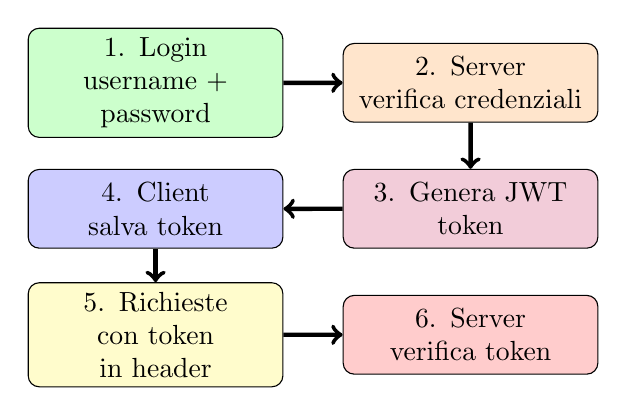
\begin{tikzpicture}[scale=0.8]
    \tikzstyle{block} = [rectangle, draw, fill=blue!20, text width=3cm, text centered, rounded corners, minimum height=1cm]
    
    % Step 1
    \node[block, fill=green!20] (login) at (0,3) {1. Login\\username + password};
    
    % Step 2
    \node[block, fill=orange!20] (server) at (5,3) {2. Server\\verifica credenziali};
    
    % Step 3
    \node[block, fill=purple!20] (jwt) at (5,1) {3. Genera JWT\\token};
    
    % Step 4
    \node[block, fill=blue!20] (client) at (0,1) {4. Client\\salva token};
    
    % Step 5
    \node[block, fill=yellow!20] (request) at (0,-1) {5. Richieste\\con token in header};
    
    % Step 6
    \node[block, fill=red!20] (verify) at (5,-1) {6. Server\\verifica token};
    
    \draw[->, ultra thick] (login) -- (server);
    \draw[->, ultra thick] (server) -- (jwt);
    \draw[->, ultra thick] (jwt) -- (client);
    \draw[->, ultra thick] (client) -- (request);
    \draw[->, ultra thick] (request) -- (verify);
\end{tikzpicture}
\end{center}

\vspace{0.3cm}
\small\textbf{JWT (JSON Web Token)}: Standard aperto (RFC 7519) per trasmettere informazioni in modo sicuro tra parti come oggetto JSON.
\end{frame}

% ====================
% SLIDE 34: Validazione Input
% ====================
\begin{frame}[fragile]{Validazione e Sanitizzazione Input}
\begin{lstlisting}[style=phpstyle, basicstyle=\ttfamily\scriptsize]
// Validazione del parametro limit
public function listAction()
{
    $arrQueryStringParams = $this->getQueryStringParams();
    
    // Valore di default
    $intLimit = 10;
    
    // Validazione
    if (isset($arrQueryStringParams['limit'])) {
        $limit = $arrQueryStringParams['limit'];
        
        // Verifica che sia un numero
        if (is_numeric($limit) && $limit > 0 && $limit <= 100) {
            $intLimit = (int)$limit;
        } else {
            // Gestione errore
            $this->sendOutput(
                json_encode(['error' => 'Invalid limit parameter']),
                ['Content-Type: application/json', 
                 'HTTP/1.1 400 Bad Request']
            );
            return;
        }
    }
    
    $arrUsers = $userModel->getUsers($intLimit);
}
\end{lstlisting}
\end{frame}

% ====================
% SLIDE 35: CORS
% ====================
\begin{frame}[fragile]{Gestione CORS (Cross-Origin Resource Sharing)}
\begin{lstlisting}[style=phpstyle, basicstyle=\ttfamily\scriptsize]
// Aggiungere in BaseController::sendOutput()

protected function sendOutput($data, $httpHeaders = array())
{
    // Headers CORS
    header('Access-Control-Allow-Origin: *');
    header('Access-Control-Allow-Methods: GET, POST, PUT, DELETE');
    header('Access-Control-Allow-Headers: Content-Type, Authorization');
    header('Access-Control-Max-Age: 3600');
    
    // Gestione preflight request
    if ($_SERVER['REQUEST_METHOD'] === 'OPTIONS') {
        http_response_code(200);
        exit();
    }
    
    header_remove('Set-Cookie');
    
    if (is_array($httpHeaders) && count($httpHeaders)) {
        foreach ($httpHeaders as $httpHeader) {
            header($httpHeader);
        }
    }
    
    echo $data;
    exit;
}
\end{lstlisting}
\end{frame}

% ====================
% SECTION 9
% ====================
\section{Estensioni e Miglioramenti}

% ====================
% SLIDE 36: Estensioni Future
% ====================
\begin{frame}{Possibili Estensioni dell'API}
\begin{columns}[T]
\column{0.5\textwidth}
\textbf{Nuovi Endpoint:}
\begin{itemize}
    \item \texttt{POST /user} - Crea utente
    \item \texttt{GET /user/\{id\}} - Dettagli utente
    \item \texttt{PUT /user/\{id\}} - Aggiorna utente
    \item \texttt{DELETE /user/\{id\}} - Elimina utente
    \item \texttt{GET /user/search} - Ricerca utenti
\end{itemize}

\vspace{0.3cm}
\textbf{Funzionalità:}
\begin{itemize}
    \item Paginazione avanzata
    \item Filtri multipli
    \item Ordinamento personalizzato
    \item Export in CSV/PDF
\end{itemize}

\column{0.5\textwidth}
\textbf{Sicurezza:}
\begin{itemize}
    \item Sistema di autenticazione
    \item Gestione ruoli e permessi
    \item Rate limiting
    \item API Key management
    \item Audit logging
\end{itemize}

\vspace{0.3cm}
\textbf{Performance:}
\begin{itemize}
    \item Redis caching
    \item Query optimization
    \item Connection pooling
    \item Async processing
\end{itemize}
\end{columns}
\end{frame}

% ====================
% SLIDE 37: Paginazione
% ====================
\begin{frame}[fragile]{Implementazione Paginazione}
\begin{lstlisting}[style=phpstyle, basicstyle=\ttfamily\tiny]
// In UserModel.php
public function getUsers($limit, $offset = 0)
{
    return $this->select(
        "SELECT * FROM users 
         ORDER BY user_id ASC 
         LIMIT ? OFFSET ?",
        ["ii", $limit, $offset]
    );
}

public function getTotalUsers()
{
    $result = $this->select("SELECT COUNT(*) as total FROM users");
    return $result[0]['total'];
}

// In UserController.php
public function listAction()
{
    $page = isset($_GET['page']) ? (int)$_GET['page'] : 1;
    $limit = isset($_GET['limit']) ? (int)$_GET['limit'] : 10;
    $offset = ($page - 1) * $limit;
    
    $userModel = new UserModel();
    $users = $userModel->getUsers($limit, $offset);
    $total = $userModel->getTotalUsers();
    
    $response = [
        'data' => $users,
        'pagination' => [
            'current_page' => $page,
            'per_page' => $limit,
            'total' => $total,
            'total_pages' => ceil($total / $limit)
        ]
    ];
    
    $this->sendOutput(json_encode($response), [...]);
}
\end{lstlisting}
\end{frame}

% ====================
% SLIDE 38: Versioning API
% ====================
\begin{frame}{Versioning dell'API}
\textbf{Strategie di versioning:}

\vspace{0.3cm}
\begin{enumerate}
    \item \textbf{URI Path:} \texttt{/api/v1/users}, \texttt{/api/v2/users}
    \item \textbf{Query String:} \texttt{/api/users?version=1}
    \item \textbf{Header:} \texttt{Accept: application/vnd.api.v1+json}
\end{enumerate}

\vspace{0.5cm}
\textbf{Esempio struttura con versioning:}
\begin{center}
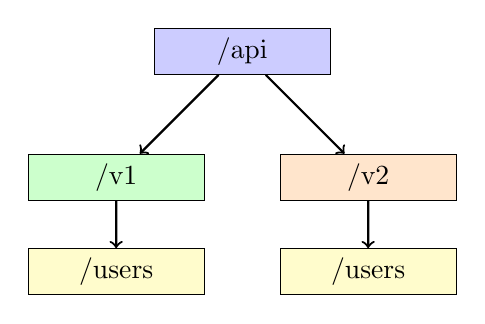
\begin{tikzpicture}[scale=0.8]
    \tikzstyle{dir} = [rectangle, draw, fill=blue!20, text width=2cm, text centered]
    
    \node[dir] (root) at (0,2) {/api};
    
    \node[dir, fill=green!20] (v1) at (-2,0) {/v1};
    \node[dir, fill=orange!20] (v2) at (2,0) {/v2};
    
    \node[dir, fill=yellow!20] (u1) at (-2,-1.5) {/users};
    \node[dir, fill=yellow!20] (u2) at (2,-1.5) {/users};
    
    \draw[->, thick] (root) -- (v1);
    \draw[->, thick] (root) -- (v2);
    \draw[->, thick] (v1) -- (u1);
    \draw[->, thick] (v2) -- (u2);
\end{tikzpicture}
\end{center}

\vspace{0.3cm}
\small Permette di evolvere l'API mantenendo retrocompatibilità.
\end{frame}

% ====================
% SLIDE 39: Documentazione API
% ====================
\begin{frame}{Documentazione dell'API}
\textbf{Strumenti per documentare REST API:}

\vspace{0.3cm}
\begin{columns}[T]
\column{0.5\textwidth}
\textbf{OpenAPI/Swagger:}
\begin{itemize}
    \item Specifica standard
    \item UI interattiva
    \item Generazione client SDK
    \item Testing integrato
\end{itemize}

\vspace{0.3cm}
\textbf{Postman:}
\begin{itemize}
    \item Collezioni condivisibili
    \item Test automatizzati
    \item Mock server
    \item Documentazione generata
\end{itemize}

\column{0.5\textwidth}
\textbf{Elementi essenziali:}
\begin{itemize}
    \item Endpoint disponibili
    \item Metodi HTTP supportati
    \item Parametri richiesti/opzionali
    \item Formato richiesta/risposta
    \item Codici di stato
    \item Esempi di utilizzo
    \item Autenticazione
    \item Rate limits
\end{itemize}
\end{columns}

\vspace{0.3cm}
\begin{exampleblock}{Best Practice}
Mantenere la documentazione sempre aggiornata con il codice!
\end{exampleblock}
\end{frame}

% ====================
% SLIDE 40: Testing Automatizzato
% ====================
\begin{frame}[fragile]{Testing Automatizzato}
\textbf{PHPUnit - Test per UserModel:}
\begin{lstlisting}[style=phpstyle, basicstyle=\ttfamily\tiny]
<?php
use PHPUnit\Framework\TestCase;

class UserModelTest extends TestCase
{
    private $userModel;
    
    protected function setUp(): void
    {
        $this->userModel = new UserModel();
    }
    
    public function testGetUsersReturnsArray()
    {
        $users = $this->userModel->getUsers(10);
        $this->assertIsArray($users);
    }
    
    public function testGetUsersRespectsLimit()
    {
        $limit = 5;
        $users = $this->userModel->getUsers($limit);
        $this->assertLessThanOrEqual($limit, count($users));
    }
    
    public function testUserStructure()
    {
        $users = $this->userModel->getUsers(1);
        $this->assertArrayHasKey('user_id', $users[0]);
        $this->assertArrayHasKey('username', $users[0]);
        $this->assertArrayHasKey('user_email', $users[0]);
        $this->assertArrayHasKey('user_status', $users[0]);
    }
}
\end{lstlisting}
\end{frame}

% ====================
% SECTION 10
% ====================
\section{Conclusioni}

% ====================
% SLIDE 41: Riepilogo Architettura
% ====================
\begin{frame}{Riepilogo dell'Architettura}
\begin{center}
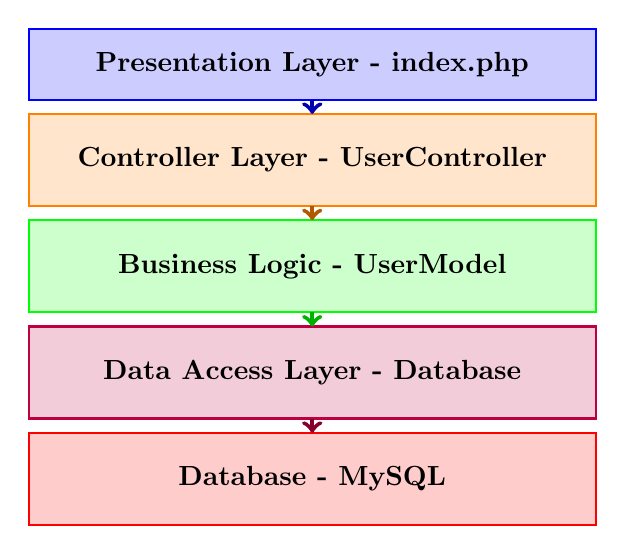
\begin{tikzpicture}[scale=0.9]
    % Layers
    \draw[fill=blue!20, draw=blue, thick] (0,4) rectangle (8,5) node[pos=.5] {\textbf{Presentation Layer - index.php}};
    
    \draw[fill=orange!20, draw=orange, thick] (0,2.5) rectangle (8,3.8) node[pos=.5] {\textbf{Controller Layer - UserController}};
    
    \draw[fill=green!20, draw=green, thick] (0,1) rectangle (8,2.3) node[pos=.5] {\textbf{Business Logic - UserModel}};
    
    \draw[fill=purple!20, draw=purple, thick] (0,-0.5) rectangle (8,0.8) node[pos=.5] {\textbf{Data Access Layer - Database}};
    
    \draw[fill=red!20, draw=red, thick] (0,-2) rectangle (8,-0.7) node[pos=.5] {\textbf{Database - MySQL}};
    
    % Arrows
    \draw[->, ultra thick, blue!70!black] (4,4) -- (4,3.8);
    \draw[->, ultra thick, orange!70!black] (4,2.5) -- (4,2.3);
    \draw[->, ultra thick, green!70!black] (4,1) -- (4,0.8);
    \draw[->, ultra thick, purple!70!black] (4,-0.5) -- (4,-0.7);
\end{tikzpicture}
\end{center}

\vspace{0.3cm}
\small\textbf{Separazione dei livelli} garantisce:
\begin{itemize}
    \item Manutenibilità del codice
    \item Testabilità dei componenti
    \item Scalabilità dell'applicazione
    \item Riutilizzo del codice
\end{itemize}
\end{frame}

% ====================
% SLIDE 42: Vantaggi Approccio REST
% ====================
\begin{frame}{Vantaggi dell'Approccio REST}
\begin{columns}[T]
\column{0.5\textwidth}
\textbf{Tecnici:}
\begin{itemize}
    \item \faCheckCircle\ Architettura scalabile
    \item \faCheckCircle\ Stateless (facilita load balancing)
    \item \faCheckCircle\ Caching ottimizzato
    \item \faCheckCircle\ Separazione client/server
    \item \faCheckCircle\ Standard HTTP universale
\end{itemize}

\vspace{0.3cm}
\textbf{Di Business:}
\begin{itemize}
    \item \faDollarSign\ Riduzione costi di sviluppo
    \item \faDollarSign\ Time-to-market più rapido
    \item \faDollarSign\ Manutenzione semplificata
\end{itemize}

\column{0.5\textwidth}
\textbf{Per gli Sviluppatori:}
\begin{itemize}
    \item \faUsers\ Codice più leggibile
    \item \faUsers\ Testing facilitato
    \item \faUsers\ Collaborazione migliorata
    \item \faUsers\ Documentazione standardizzata
\end{itemize}

\vspace{0.3cm}
\textbf{Per gli Utenti:}
\begin{itemize}
    \item \faHeart\ Performance migliori
    \item \faHeart\ Esperienza multi-dispositivo
    \item \faHeart\ Affidabilità superiore
\end{itemize}
\end{columns}
\end{frame}

% ====================
% SLIDE 43: Punti Chiave
% ====================
\begin{frame}{Punti Chiave del Tutorial}
\begin{enumerate}
    \item \textbf{REST API} sono lo standard de facto per servizi web moderni
    \item \textbf{PHP 8} offre strumenti potenti per implementare API robuste
    \item \textbf{Pattern MVC} separa responsabilità e migliora manutenibilità
    \item \textbf{Prepared Statements} proteggono da SQL Injection
    \item \textbf{Routing URI} permette endpoint puliti e RESTful
    \item \textbf{Gestione errori} fornisce feedback chiari ai client
    \item \textbf{JSON} è il formato standard per lo scambio dati
    \item \textbf{Estensibilità} è garantita dalla struttura modulare
\end{enumerate}

\vspace{0.5cm}
\begin{alertblock}{Ricorda}
Questo è solo l'inizio! Le REST API possono essere molto più complesse e potenti.
\end{alertblock}
\end{frame}

% ====================
% SLIDE 44: Risorse Aggiuntive
% ====================
\begin{frame}{Risorse per Approfondire}
\textbf{Documentazione Ufficiale:}
\begin{itemize}
    \item PHP: \url{https://www.php.net/manual/}
    \item MySQL: \url{https://dev.mysql.com/doc/}
    \item REST API: \url{https://restfulapi.net/}
\end{itemize}

\vspace{0.3cm}
\textbf{Framework PHP per API:}
\begin{itemize}
    \item Laravel (con Passport/Sanctum)
    \item Symfony (con API Platform)
    \item Slim Framework
    \item Lumen
\end{itemize}

\vspace{0.3cm}
\textbf{Strumenti Utili:}
\begin{itemize}
    \item Postman - Testing API
    \item Swagger/OpenAPI - Documentazione
    \item Docker - Containerizzazione
    \item Git - Version Control
\end{itemize}
\end{frame}

% ====================
% SLIDE 45: Esercizi Pratici
% ====================
\begin{frame}{Esercizi Proposti}
\textbf{Livello Base:}
\begin{enumerate}
    \item Aggiungere un endpoint per recuperare un singolo utente per ID
    \item Implementare filtri per user\_status nella lista utenti
    \item Aggiungere ordinamento personalizzato (ASC/DESC)
\end{enumerate}

\vspace{0.3cm}
\textbf{Livello Intermedio:}
\begin{enumerate}
    \item Implementare endpoint POST per creare nuovi utenti
    \item Aggiungere validazione email con regex
    \item Implementare sistema di paginazione completo
\end{enumerate}

\vspace{0.3cm}
\textbf{Livello Avanzato:}
\begin{enumerate}
    \item Implementare autenticazione JWT
    \item Creare sistema di rate limiting
    \item Aggiungere logging delle richieste
    \item Implementare cache con Redis
\end{enumerate}
\end{frame}

% ====================
% SLIDE 46: Domande?
% ====================
\begin{frame}
\begin{center}
\Huge\textbf{Domande?}

\vspace{1cm}

\Large
\faEnvelope\ \href{mailto:prof@example.com}{prof@example.com}

\vspace{0.5cm}

\faGithub\ \href{https://github.com}{github.com/username}

\vspace{1cm}

\large
\textit{Grazie per l'attenzione!}

\vspace{1cm}

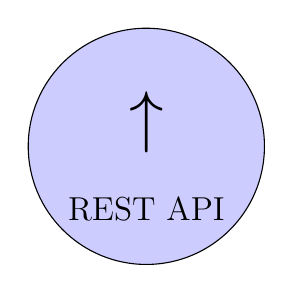
\begin{tikzpicture}
    \node[draw, circle, fill=blue!20, minimum size=3cm] (thanks) at (0,0) {};
    \node at (0,0.3) {\Huge\faThumbsUp};
    \node at (0,-0.8) {\large REST API};
\end{tikzpicture}
\end{center}
\end{frame}

\end{document}
